\shorthandoff{"}
\chapter{Verwandte Arbeiten}
\label{ch:verwandteArbeiten}
Bei der Durchsicht der Literatur ist festzustellen, dass bereits zahlreiche Publikationen den Anspruch verfolgten, bilaterale Systeme zur automatisierten Bestimmung des \acp{PJFit} zu entwickeln. Jedoch bezogen sich einige Forscher dabei nicht auf das in Kapitel \ref{ch:personEnvironmentFit} vorgestellte Konzept der Psychologie. Obwohl der Begriff des \acp{PJFit} verwendet wurde, bestimmten die Wissenschaftler die Kongruenz häufig ausschließlich auf der Ebene des Anforderungen-Fähigkeiten Fits. Dieser Sachverhalt ist beispielsweise in den Veröffentlichungen von \textcite[S. 1ff.]{luo:2019}, \textcite[S. 1ff.]{qin:2018} und \textcite[S. 1ff.]{personJobFit:2018} zu beobachten.

\section{Nicht auf dem PE-Fit basierende Systeme}
\label{ch:verwandteArbeiten:nichtAufDemPEFitBasierend}
\textcite[S. 1, Z. 1f.]{personJobFit:2018} definierten den \ac{PJFit} als den "Prozess, bei dem das richtige Talent mit der richtigen Stelle zusammengeführt wird, indem die Talentkompetenzen identifiziert werden, welche für die Stelle erforderlich sind."\footnote{"process of matching the right talent for the right job by identifying talent competencies that are required for the job." - \textcite[S. 1, Z. 1f.]{personJobFit:2018}} Dementsprechend stellten die Wissenschaftler in ihrer Publikation ein System vor, welches über modellbasierte Verfahren aus unstrukturierten Bewerbungsdaten lernte, ob eine Person aufgrund ihrer Fähigkeiten für die Anforderungen einer Stelle geeignet ist \cite[S. 1ff.]{personJobFit:2018}. Ähnliche Systeme entwickelten auch \textcite[S. 1ff.]{qin:2018} und \textcite[S. 1ff.]{luo:2019}. In beiden Fällen bereiteten die Wissenschaftler Stellenausschreibungen und Lebensläufe durch modellbasierte Verfahren strukturiert auf. Diese Daten nutzten die Forscher, um über ein neuronales Netz vorauszusagen, ob eine ausreichende Übereinstimmung zwischen den Fähigkeiten der Kandidaten und den Anforderungen der offenen Stellen vorhanden ist. 

Empfehlungssysteme, welche neben dem Anforderungen-Fähigkeiten Fit auch den Bedürfnisse-Angebote Fit betrachten, bezeichneten \textcite[S. 4]{malinowski:2006} als bilaterale Empfehlungssysteme. Im Umfeld dieser Wissenschaftler entwickelten verschiedene Forschergruppen zwei Recommender Engines, welche in mehreren Publikationen vorgestellt wurden. In beiden Fällen bezogen sich die Wissenschaftler auf das in Kapitel \ref{ch:personEnvironmentFit} vorgestellte Konzept des \acp{PEFit} \cite[S. 4f.]{keim:2007}\cite[S. 3f.]{keim:2005}\cite[S. 3f.]{malinowski:2005}\cite[S. 3f.]{malinowski:2006}\cite[S. 3ff.]{malinowski:2008}.

\section{Auf dem PE-Fit basierende bilaterale Systeme}
\label{ch:verwandteArbeiten:aufDemPEFitBasierendeBilateraleSysteme}
Eine der beiden Anwendungen aus dem Umfeld von \textcite[S. 1ff.]{malinowski:2006} verfolgte das Ziel, neue Personen für bestehende Teams zu empfehlen. Zu diesem Zweck sagten die Wissenschaftler vorher, wie sehr sich potentielle Teammitglieder gegenseitig vertrauen würden. Dabei schlugen sie diejenigen Kandidaten für das Team vor, bei welcher der höchste gegenseitige Vertrauenswert zwischen bestehenden Teamkollegen und potentiellem Mitglied berechnet wurde \cite[S. 5ff.]{keim:2005}\cite[S. 1ff.]{malinowski:2005}. Das zweite System sollte Empfehlungen zur Besetzung offener Stellen generieren und dabei Präferenzen von Arbeitssuchenden und Personalsachbearbeitern beachten \cite[S. 1ff.]{malinowski:2006}. Darüber hinaus stellte \textcite[S. 5ff.]{keim:2007} ein System vor, welches beide Ansätze innerhalb einer Anwendung integrierte. Alle diese Implementierungsmethoden basieren auf einem von \textcite[S. 6ff.]{faerber:2003} vorgestellten Empfehlungssystem.

\textcite[S. 4ff.]{faerber:2003} entwickelten eine Recommender Engine zur Empfehlung von Personen für offene Stellen in Unternehmen. Dabei verfolgten sie einen hybriden, nicht-bilateralen Ansatz. Dieser ist in Abbildung \ref{fig:verwandteArbeiten:abb1} modelliert.

\begin{figure}[h]
	\centering
	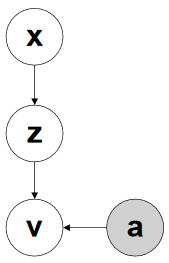
\includegraphics[width=0.3\textwidth]{gfx/faerber.png}
	\caption{Modell des hybriden Empfehlungssystems von \textcite[S. 8]{faerber:2003}}
	\label{fig:verwandteArbeiten:abb1}
\end{figure}

In Abbildung \ref{fig:verwandteArbeiten:abb1} steht $a$ für die Attribute des Bewerbers, welche beispielsweise aus dessen Lebenslauf gewonnen wurden. Variable $x$ symbolisiert einen Personalsachbearbeiter mitsamt eines Stellenprofils, welches dieser besetzen soll. Dessen Entscheidung, ob ein Bewerber für die Tätigkeit qualifiziert ist oder nicht, wurde über den boolschen Wert $v$ ausgedrückt. \textcite[S. 4ff.]{faerber:2003} bestimmten aus diesen Faktoren ein latentes Variablenmodell. Hierbei wurden aus bekannten Entscheidungen eines Personalsachbearbeiters $x$ hinsichtlich der Eignung $v$ eines Bewerbers $a$ für eine Stelle nicht direkt messbare Variablen $z$ abgeleitet, welche dessen Beurteilungen beeinflussten. Über die latenten Variablen $z$ und die Attribute $a$ bestimmten die Wissenschaftler Wahrscheinlichkeiten, mit welchen ein Personalsachbearbeiter die vorliegenden Attribute eines Kandidaten als qualifiziert oder unqualifiziert bewerten würde.

In ihrer Publikation erweiterten \textcite[S. 4f.]{malinowski:2006} das von \textcite[S. 4ff.]{faerber:2003} entwickelte Verfahren. Hierbei verfolgten die Wissenschaftler das Ziel, zusätzlich zur Empfehlung von Kandidaten für Arbeitsplätze auch Stellen für Arbeitssuchende passend zu deren Vorlieben zu empfehlen. Dazu ergänzten sie eine weitere Komponente für Stellensuchende im System, welche sich ebenfalls am Aufbau von Abbildung \ref{fig:verwandteArbeiten:abb1} orientierte. Bei der neuen Komponenten stand $x$ für den Kandidaten und $a$ für die Attribute der Stellenausschreibung. Auch hier bestimmten die Forscher latente Variablen $z$, welche sie über vergangene Stellenprofil-Bewertungen von Studenten ermittelten. Über diese sagten sie voraus, mit welcher Wahrscheinlichkeit ein Kandidat eine Stelle als passend zu seinen Präferenzen bewerten würde.

Bei einer Evaluation des Systems stellten \textcite[S. 6f.]{malinowski:2006} fest, dass die Ergebnisse der Komponente zur Empfehlung von Kandidaten nahezu vergleichbar zur manuellen Auswahl eines menschlichen Personalsachbearbeiters war. Auch beim Stellenempfehlungssystem kamen die Wissenschaftler zu der Erkenntnis, dass deren Ergebnisse bis auf einzelne Ausnahmen vergleichbar zur manuellen Auswahl der Kandidaten waren. Auch \textcite[S. 7]{keim:2007} bestätigte, dass beide Empfehlungsmodule eine hohe Genauigkeit aufweisen konnten.

Zu diesem Vorgehen von \textcite[S. 3ff.]{malinowski:2006} ist festzustellen, dass das bilaterale Empfehlungssystem ursprünglich in Anlehnung an das Konzept des \acp{PEFit} entwickelt wurde. Dabei sollten sowohl Präferenzen von Personalsachbearbeitern als auch Vorlieben von Stellensuchenden berücksichtigt werden. Allerdings ist es in der vorgestellten Anwendung nur möglich, entweder zu den Präferenzen von Personalsachbearbeitern passende Kandidaten oder mit den Vorlieben von Bewerbern kompatible Stellen zu ermitteln. Es ist nicht vorgesehen, Kandidaten für Positionen zu empfehlen und dabei gleichzeitig die Präferenzen von Bewerbern und Personalsachbearbeitern zu berücksichtigen. Daher ist kritisch anzumerken, dass die Anwendung von \textcite[S. 3ff.]{malinowski:2006} zwar die Präferenzen beider Parteien berücksichtigte, dieses Vorgehen aber nicht vollständig der Theorie des \acp{PEFit} entspricht.

In einer weiteren Veröffentlichungen präsentierten \textcite[S. 1]{malinowski:2005} ein Empfehlungssystem, welches Personen für Teams vorschlagen sollte. Einerseits berücksichtigten die Wissenschaftler hierbei die Präferenzen von Personalsachbearbeitern hinsichtlich der fachlichen Eignung der Kandidaten berücksichtigt. Andererseits beachteten sie auch die Präferenzen von Teammitgliedern und potentiellem Kandidaten bezüglich der persönlichen Zusammenarbeit.

Um dieses Ziel zu erreichen, sah es das System von \textcite[S. 4ff.]{malinowski:2005} in einem ersten Schritt vor, über das Verfahren von \textcite[S. 8ff.]{faerber:2003} aus allen verfügbaren Personen die $N$ fachlich geeignetsten Kandidaten passend zu den Präferenzen des Personalsachbearbeiters zu bestimmen. Diese dienten als Eingabe für eine weitere Komponente, über welche die Wissenschaftler das potentielle Vertrauen zwischen den $N$ Kandidaten und den vorhanden Teammitgliedern berechneten. Um das Vertrauen zu bestimmen, nutzten die Forscher drei separate Ansätze. Diese sind in Abbildung \ref{fig:verwandteArbeiten:abb2} dargestellt und wurden auch in den Publikationen von \textcite[S. 5ff.]{keim:2005} und \textcite[S. 6ff.]{malinowski:2008} vorgestellt.

\begin{figure}[h]
	\centering
	
	\subfloat[Transitive Beziehung]{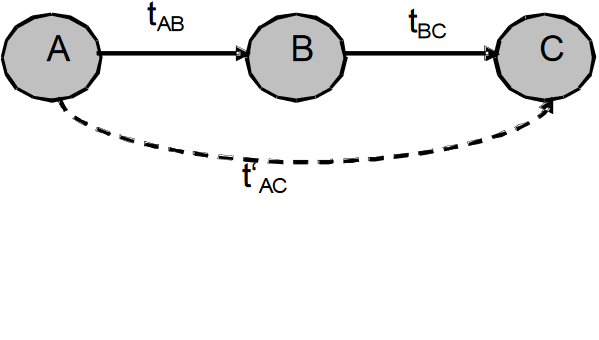
\includegraphics[width = 0.33\textwidth]{gfx/trustmodelA.png}}
	\subfloat[Kollaboratives Filtern]{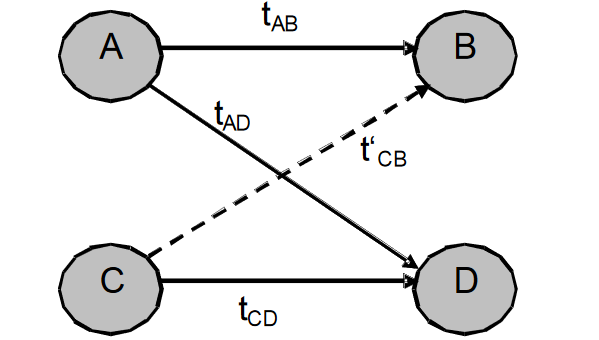
\includegraphics[width = 0.33\textwidth]{gfx/trustmodelB.png}}
	\subfloat[Ähnlichkeitsberechnung über latente Variablen]{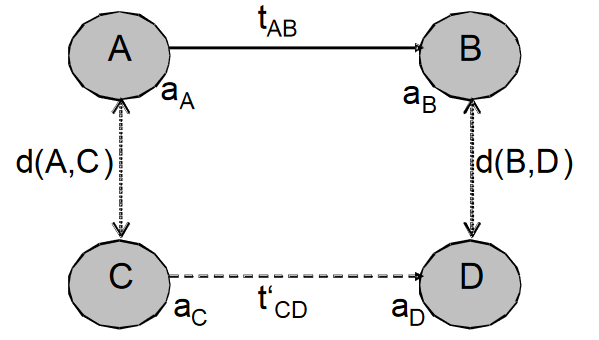
\includegraphics[width = 0.33\textwidth]{gfx/trustmodelC.png}}
	
	\caption{Ansätze zur Berechnung des Vertrauens zwischen Teammitgliedern \cite[S. 5]{malinowski:2005}}
	\label{fig:verwandteArbeiten:abb2}
\end{figure}

Die Anwendung der ersten beiden Ansätze (a) und (b) zur Vorhersage des Vertrauens zwischen potentiellen Teammitgliedern aus Abbildung \ref{fig:verwandteArbeiten:abb2} setzt laut \textcite[S. 4ff.]{malinowski:2005} voraus, dass bekannte Vertrauensbewertungen von Teamkollegen vorhanden sind. Diese können den Wissenschaftlern zu Folge beispielsweise über Fragebögen ermittelt werden.

Bei Ansatz (a) nahmen \textcite[S. 5f.]{malinowski:2005} an, dass eine Vertrauensbeziehung über Multiplikation berechnet werden kann, wenn transitiv eine direkte Beziehung zwischen zwei Personen besteht. Zur Berechnung der Vertrauensbeziehung $t'_{AC}$ von Person A zu Person C wendeten die Wissenschaftler folgende Formel \ref{frml:verwandteArbeiten:formel1} an:
\begin{equation}
	t'_{AC} = t_{AB} * t_{BC}
	\label{frml:verwandteArbeiten:formel1}
\end{equation}
Ansatz (b) in Abbildung \ref{fig:verwandteArbeiten:abb2} zeigt die Berechnung des Vertrauens zwischen zwei Personen über speicherbasiertes kollaboratives Filtern wie es in Kapitel \ref{ch:empfehlungssysteme:cf} vorgestellt wurde. Hierbei wurde die Ähnlichkeit zwischen Person A und Person C genutzt, um den Vertrauenswert zwischen Person C und Person B vorherzusagen \cite[S. 6]{malinowski:2005}.

Das dritte Verfahren (c) beruhte auf der Annahme, dass sich Personen stark vertrauen würden, wenn sie ähnliche persönliche Präferenzen teilen. Unter dieser Prämisse erstellten \textcite[S. 6f.]{malinowski:2005} ein latentes Variablenmodell vergleichbar zu Abbildung \ref{fig:verwandteArbeiten:abb1}. Über dieses bestimmten sie für jedes Teammitglied diejenigen latenten Variablen, welche für dieses bei der Bewertung vergangener Stellen besonders wichtig waren. Die ermittelten latenten Variablen und die gemeinsam bewerteten Stellenprofile nutzen die Wissenschaftler, um über die Ähnlichkeit zwischen Personen auf deren gegenseitiges Vertrauen zu schließen.

Die aus den drei Ansätzen (a), (b) und (c) erhaltenen Vertrauenswerte zwischen bestehenden Teammitgliedern und potentiellen Kandidaten aggregierten \textcite[S. 7ff.]{malinowski:2005} unter Berücksichtigung der Anzahl gemeinsam bewerteter Stellenprofile zu einer finalen Vertrauensbewertung.

Im letzten Schritt des Systems errechneten \textcite[S. 9f.]{malinowski:2005} aus den Ergebnissen der Komponente von \textcite[S. 8ff.]{faerber:2003} und der finalen Vertrauensbewertung eine Ergebnisliste. Hierzu wendeten sie die folgende Formel \ref{frml:verwandteArbeiten:formel2} an:
\begin{equation}
	R' = \alpha * t'_{M*y} * (1-\alpha) * r'_{x,y,v}
	\label{frml:verwandteArbeiten:formel2}
\end{equation}
In Formel \ref{frml:verwandteArbeiten:formel2} stand $t'_{M*y}$ für die Liste der Vertrauensbeziehungen und $r'_{x,y,v}$ für die fachlichen Bewertungen der Kandidaten. Für $\alpha$ setzten die Wissenschaftler den Wert 0.5 ein \cite[S. 4ff.]{malinowski:2005}. Jedoch merkten \textcite[S. 9]{malinowski:2005} zu Formel \ref{frml:verwandteArbeiten:formel2} an, dass diese noch nicht optimal sei und weiterer Forschung bedarf.

Eine Evaluation des Gesamtsystems konnte in der Literatur nicht identifiziert werden. In der Publikation von \textcite[S. 13ff.]{malinowski:2008} findet sich jedoch eine Validierung der Komponente zur Berechnung des Vertrauens zwischen Teammitgliedern und potentiellen Kandidaten. Hierbei kamen die Wissenschaftler zu der Erkenntnis, dass deren System eine höhere Genauigkeit als ein zufälliges Vorhersagesystem aufweisen konnte. Allerdings merkten die Forscher zu ihrer Testgruppe an, dass diese mit 21 Teilnehmern zu klein sei, um signifikante Resultate zu bieten.

In einer weiteren Veröffentlichung stellte \textcite[S. 1ff.]{keim:2007} in Ergänzung zu den vorherigen Anwendungen von \textcite[S. 6ff.]{faerber:2003}, \textcite[S. 4ff.]{keim:2005}, \textcite[S. 4ff.]{malinowski:2005} und \textcite[S. 3ff.]{malinowski:2006} das in Abbildung \ref{fig:verwandteArbeiten:abb3} dargestellte Framework vor. Dieses verfolgte das Ziel, Kandidaten in passende Projektteams einzuordnen und dabei sowohl Fähigkeiten als auch zwischenmenschliche Attribute zu berücksichtigen \cite[S. 1ff.]{keim:2007}.

\begin{figure}[h]
	\centering
	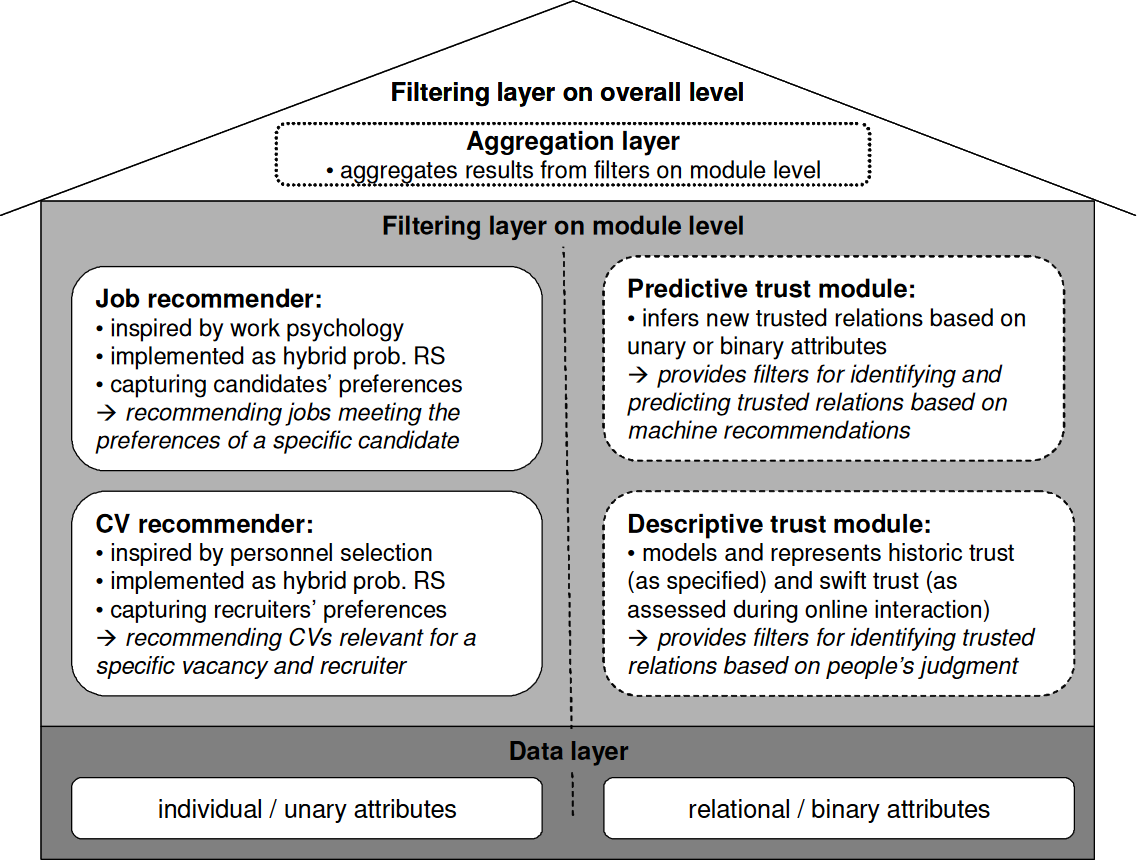
\includegraphics[width=0.8\textwidth]{gfx/keim-multilayer.png}
	\caption{Das Empfehlungssystem von \textcite[S. 5]{keim:2007}}
	\label{fig:verwandteArbeiten:abb3}
\end{figure}

In Abbildung \ref{fig:verwandteArbeiten:abb3} ist zu erkennen, dass die zweite Ebene des Empfehlungssystems von \textcite[S. 5ff.]{keim:2007} aus vier Komponenten bestand. Diese sollten die Daten, welche auf der ersten Ebene gespeichert wurden, laden und entsprechend ihrer Funktion filtern. Dabei sollten die beiden auf der linken Seite abgebildeten Module die Stellen- bzw. Kandidatensuche unterstützen. Die Komponenten der rechten Seite sollten die Suche nach geeigneten Teampartnern erleichtern.

Das Lebenslaufempfehlungssystem (CV recommender) in Abbildung \ref{fig:verwandteArbeiten:abb3} entsprach der von \textcite[S. 8ff.]{faerber:2003} entwickelten Anwendung, welche anhand von Abbildung \ref{fig:verwandteArbeiten:abb1} vorgestellt wurde \cite[S. 6]{keim:2007}. Beim Stellenempfehlungssystem (Job recommender) handelte es sich um die von \textcite[S. 4ff.]{malinowski:2006} adaptierte Version des Lebenslaufempfehlungssystems mit welcher Personen zu ihren Präferenzen passende Stellenausschreibungen ermitteln konnten \cite[S. 6]{keim:2007}. Das vorhersagende Vertrauensmodul (Predictive Trust module) entsprach dem anhand von Abbildung \ref{fig:verwandteArbeiten:abb2} behandelten Ansatz zur Vorhersage von Vertrauensbeziehungen zwischen potentiellen Teammitgliedern \cite[S. 8]{keim:2007}. Dieses wurde in den Publikationen von \textcite[S. 5ff.]{keim:2005} und \textcite[S. 4ff.]{malinowski:2005} detailliert vorgestellt. Vergleichbar zu einer in der Veröffentlichung von \textcite[S. 4f.]{keim:2005} vorgestellten Anwendung ist auch das beschreibende Vertrauensmodul (Descriptive trust module). Diese Komponente erfasste explizit vergebene Vertrauensbewertungen von Teammitgliedern in Form einer Ontologie und repräsentiert diese in Form eines Graphen. Über diese Darstellung konnten Anwender soziale Beziehungen durchsuchen und analysieren. Auf diese Weise sollten sie besser entscheiden können, mit welchen Personen sie eine Zusammenarbeit eingehen möchten \cite[S. 7]{keim:2007}.

Ähnlich zur Publikation von \textcite[S. 3ff.]{malinowski:2006} muss auch zur Veröffentlichung von \textcite[S. 5ff.]{keim:2007} kritisch bemerkt werden, dass die Forscher die Resultate der einzelnen Module nicht zu einem Ergebnis zusammenfassten. Die Implementierung der oben in Abbildung \ref{fig:verwandteArbeiten:abb3} dargestellten Aggregationsebene (Aggregation layer) ließen die Wissenschaftler in ihrer Publikation offen \cite[S. 8]{keim:2007}.
%Das von \textcite{keim:2007} vorgestellte System enthielt mit dem beschreibenden und dem vorhersagenden Vertrauensmodul somit zwar Komponenten, welche bilaterale Vertrauensbeziehungen modellieren bzw. bei der Empfehlungsbestimmung berücksichtigten. Damit handelte es sich bei der Suche nach potentiell vertrauenswürdigen Teamkollegen um einen bilateralen Prozess, da Präferenzen von bestehenden Teammitgliedern und potentiellen Kandidaten berücksichtigt wurden. Es wurde jedoch nicht beachtet, ob die Person auch fachlich für die Stelle geeignet war oder ob die Position inhaltlich den Vorstellungen des Kandidaten entsprach.

Zusammenfassend ist zu den Publikationen aus dem Umfeld von \textcite[S. 4]{malinowski:2006} festzustellen, dass diese zahlreiche einzelne Empfehlungssysteme entwickelten. Diese unterstützten insbesondere die Auswahl fachlich geeigneter Stellen bzw. Kandidaten und die Zusammenführung von Personen in bestehende Teams. Bei der Implementierung dieser Systeme bezogen sich die Wissenschaftler auf das Konzept des \acp{PEFit}. Jedoch muss kritisch bemerkt werden, dass die einzelnen Module nur in Kombination tatsächlich bilaterale Empfehlungen generieren können. Die Integration verschiedener Ansätze wurde jedoch ausschließlich in der Publikation von \textcite[S. 4ff.]{malinowski:2005} vorgenommen. Hierbei wurden Kandidaten entsprechend der fachlichen Präferenzen von Personalsachbearbeitern ausgewählt und unter Beachtung des gegenseitigen Vertrauens mit den potentiellen Teammitgliedern sortiert. In den Publikationen der Forscher konnte jedoch keine Methode identifiziert werden, bei welcher eine Anwendung Stellen passend zu den fachlichen Präferenzen von Personalsachbearbeitern und Kandidaten bestimmte. Außerdem ist festzustellen, dass die Wissenschaftler ihre Systeme zwar evaluieren. Hierbei prüften sie jedoch ausschließlich, ob die Ergebnisse ihrer Anwendungen vergleichbar mit den Entscheidungen von Menschen waren. Hierbei hinterfragten sie jedoch nicht, ob die Auswahl der Nutzer tatsächlich optimal war und es somit grundsätzlich erstrebenswert war, diese Entscheidungen maschinell nachzubilden. Außerdem validierten die Forscher nicht, ob die Ergebnisse bilateraler Empfehlungssysteme tatsächlich besser sind als die Resultate der unilateralen Vorgehen. Somit bleibt ungewiss, ob der im Vergleich zu den in Kapitel \ref{ch:empfehlungssysteme} vorgestellten Anwendungen höhere Implementierungsaufwand für bilaterale Systeme in er Praxis gerechtfertigt ist.

\textcite{ding:2016}

\section{Nicht auf dem PE-Fit basierende bilaterale Systeme}
\label{ch:verwandteArbeiten:nichtAufDemPEFitBasierendeBilateraleSysteme}
 

\newpage
\textcite{ding:2016}:\\
S. 1:\\
- Entwickelten ein wechselseitiges Empfehlungssystem zum Recruitment von Absolventen
- Nutzt dafür historische Daten der Universität über Absolventen und frühere Absolventen
- Nutzen CF und CB
- System betrachtet Anforderungen von Absolventen UND Arbeitgebern
- Nutzt historische Informationen der Universität über Absolventen und frühere Absolventen --> Verbessert Genauigkeit
- Anmerkung von mir: Ist zwar wechselseitig, bezieht sich aber nicht auf den P-E Fit

S. 2\\
- Es gibt 2 Arten von Nutzern: Arbeitgeber und aktuelle Absolventen (Jobsuchende)
- Jobsuchende können grundlegende Informationen und Job-Präferenzen in das Recommender System eingeben / Nach Registrierung liest RS automatisch ihre Bildungsinformationen aus dem historischen Daten-Repository
- Arbeitgeber können grundlegende Informationen über Job-Anforderungen eingeben / Nach Registierung liest RS automatisch alle Bildungsinformationen ehemaliger Absolventen, welche in den letzten drei Jahren bei diesem Arbeitgeber angefangen haben
- Danach hilft RRSGR die richtigen Bewerber an den Arbeitgeber zu empfehlen
- Für Absolventen g hilft RRSGR ähnliche ehemalige Absolventen zu finden, welche ähnihce Performance wie g während ihrer Universitätszeit hatten --> Dann kombiniert mit den Jobs aus dem Internet und Jobs von den ehemaligen Absolventen, hilft RRSGR eine Job-Liste für g zu erstellen --> Als letztes priority k-medoids clustering hilft, die meist repräsentativen k jobs auszuwählen und diese auf dem Bildschirm des Nutzers anzuzeigen
- Für Arbeitgeber wird RRSGR helfen die ehemaligen Absolventen zu finden, welche vom Arbeitgeber von dieser Universität in den letzten drei Jahren angestellt wurden --> Dann hilft RRSGR Kandidaten zu finden, welche eine ähnliche Performance mit den angestellten ehemaligen Studenten aufweist --> Als letztes werden die meist repräsentativen k Absolventen an den Arbeitgeber empfohlen

S. 3\\
- Jede Entität hat ein Profil; Zwei Entitäten können über korrespondierende Felder in ihren Profilen verglichen werden; Manche wichtigen Felder werden ausgewählt um die Ähnlihckeit zwischen zwei Entitäten zu bestimmen
- Ähnlichkeit zwischen zwei Entitäten kann über die gewichtete Summe der Ähnlichkeit jedes korrespondierenden Feldes bestimmt werden
- Um die Diversität zu erhöhen, wählt RRSGR nicht die top k Entitäten im Sinne der Nachbarschafts-Selektion aus --> Binary Trees helfen, zu alleviate überspezifikation und concentration bias
- Priority k-medoids Clustering: Zur Erhöhung der Diversität bei der Auswahl der k Empfehlungen --> Implementiert über priority cover-tree --> Balance zwischen hohem Rank und Diversität

- Vergleich in Evaluation mit content-based Profile-Similarity (CPS) und CCR und iHR werden mit RRSGR vergleichen / Performance vergleichbar mit iHR --> RRSGR kann aber mehr Diversität bieten

\textcite{wenxing:2015}\\
S. 1\\
- Mobil Reciprocal Job Recommender System, genannt iHR+
- Teilten Features von Job-Suchenden und Jobs in zwei Kategorien, eine zur Selbst-Beschreibung des Job-Suchenden oder einen Job un ddie andere präsentiert die Präferenzen von ihnen
- Bi-Directionale Präferenz basiert auf Cross-Similarity und wurde dann berechnet, um eine reciprocale Empfehlung zu erhalten
- Wechselseitiges Empfehlungssystem erstmals vorgestellt von Pizzato et al

S. 2\\
- Relationen unter Nutzern werden über cross-similarity modelliert, welche indizieren die bi-directionale Präferenz zwischen denen
- Es gibt zwei Sets von Nutzern: Job-Suchende J und Recruiter R; Jeder Nutzer hat eine Selbst-Beschreibung Fs und eine Präferenz Fp, welche beschreibt, was er bevorzugt
- Cross-Similarity: Es gibt einen Jobsuchenden j und einen Recruiter r --> die Präferenz von j zu r (Pjr) ist definiert als die Ähnlichkeit zwischen $F_j^p$ und $F_r^s$; Die Präferenz von r zu j (Prj)ist definiert als die Ähnlichkeit zwischen Präferenz des Recruiters und Selbstbeschreibung es Suchenden / Bidirektionale Präferenz CS zwischen j und r ist definiert als die gewichtete Summe von Pjr und Prj

- Kosinus-Ähnlichkeit
- Zuerst werden die basic Features der Nutzer extrahiert --> Dann Features in Vektoren

S. 3\\
- Dann Ähnlichkeitsberechnung
- Anmerkung von mir: Keine Evaluation und keine Anlehnung an P-E Fit, trifft es aber

\textcite{oezcan:2016}\\
S. 1\\
- Wechselseitiges Empfehlungssystem CCRS --> Es können Job-Angebote veröffentlicht weren; Kandidaten können wechselseitig Feedback erhalten, durch das Nutzerprofil, Interaktion und Präferenz-Information und alles zusammen

S. 2\\
- Kandidatenprofil besteht aus 19 Merkmalen

S. 3\\
- Zusätzlich gibt es 9 weitere Merkmale, Reflektieren die Aktionen der job-Ausschreibenden Unternehmen auf dem CV des Kandidaten (z.B. CV geöffnet, gedruckt, etc.)
- Und es gibt Job-Profil Features (z.B. Ort, Unternehmen, Sektor, etc.)

- Empfehlungserstellung für den Kandidaten: 1. Die 10 Prozent ähnlichsten Kandidaten zum Kandidat werden bestimmt --> Wenn es kein Cod Start ist, wird auch der Kandidat selbst zur Liste hinzugefügt --> Danach werden die vorherigen Job, auf welche die Kandidaten der Kandidatenliste sich beworben haben werden in eine Job-Liset hinzugefügt --> Zusätzlich werden die ersten 1 Prozent der ählichsten Jobs zu den Jobs in der Jobliste zur Jobliste hinzugefügt / Verwendung der Kosinus-Ähnlichkeit

S. 4\\
- Der Rückgabe-Wert der Jobs in der Liste wird über die Interaktionen auf den CVs der Personen bestimmt, welche sich auf einen Job beworben haben --> Dieser Label-Wert wird für jeden Job über Methoden der Klassifikation und die Antwort der Jobs in der Jobliste, die wahrscheinlich gesendet wird, wird über diese Art berechet --> Ziel-Kandidaten-Feedback-Wert der Jobs wird als FB bezeichnet --> So erhält man die Information, ob sie den Zielkandidaten für jeden Job in der Liste bevorzugen werden
- Merke: Man versucht hier vorherzusagen, wie die Unternehmen reagieren werden, wenn sich der Zielkandidat auf den Job bewoibt --> Dazu werden die Interaktionen auf den CVs analysiert, welche sich kürzlich für den Job beworben haben --> Anwort wird über Klassifikation bestimmt --> JoblistFB
- Dann wird noch ein Importance Wert für die Jobs erstellt --> Für jeden Kandidaten wird ein Konfidenzwert berechnet, indem die Bewerbungen im System, welche kürzlich carried out von den Kandidaten wurden --> Konfidenzwert wird über die Ähnlichkeit zu Jobs bestimmt, auf welche sich ein Kandidat beworben hat --> Ist die Ähnlichkeit zwischen den Jobs, auf die sich ein Kandidat beworben hat, sehr hoch, ist der Konfidenzwert für diesen Kandidaten hoch --> Jeder Kandidat bietet seinen Konfidenz-Wert an den Job, an den er sich beworben hat --> Wichtigkeitswert der Jobs wird über die Summe der Kandidaten bestimmt, welche sich auf diesen Job beworben haben --> Diese wichtigkeitswerte werden als Score Wert der Jobs und Namen als SV akzeptiert --> Ein Score Value wird für jeden Job in der JobList (JobListScore) geboten
- FB-Wert und SV-Werte jedes Jobs werden multipliziert und die Jobs werden den Zielkandidaten nach diesen Werten präsentiert

S. 6\\
- CCRS zeigte in der Evaluation eine bessere Performance im Vergeich zu anderen Systemen wie iHR+

\textcite{buettner:2014}:\\
S. 1\\
- Bezug auf Person-Organization Environment fit
- Zeigt, wie Informationen aus Sozialen Netzwerken genutzt werden können, um einen P-OE fit zu bestimmen
- Kritik: Soziale Interaktionen werden von bestehenden Systemen kaum betrachtet
- Betrachtet auch das Match zwischen Persönlichkeit des Bewerbers un der Organisationskultur

S. 2\\
- Maurer und Cook (3): Zeigen, dass P-OE fit eine Schlüsselrolle bei der Qualität von Bewerbungen spielt

S. 3\\
- Diese Arbeit beachtet beim P-J Fit nur demands-abilities

S. 6\\
- In Ergänzung zu Malinowski betrachtet dieser Autor auch den Culture-Fit --> Malinowski richtete sich nur an Unternehmensinternes Staffing
- Kombiniert CB mit CF für Online Soziale Netzwerke Recruiting / Content Based
- System erhält als Input einen Kandidaten und eine Stelle und gibt eine echte Zahl zurück --> Wird in drei Sub-Funktionen unterteilt: P-O, P-G, P-J und einer Aggregierungsfunktion A --> Kombiniert diese sub-Funktionen über die aggregation der relativen Wichtigkeit placed on the sub-fits

S. 7\\
- Aggregation-Funktion A stellt ein Multi Criteria Decision Making (MCDM) Problem da --> Problem: Ein sehr niedriger Wert kann durch einen sehr hohen Wert ausgeglichen werden
- Gutes Bild zum Ansatz
- Anmerkung von mir: Hat System nicht implementiert

\textcite{hong:2013}\\
S. 1:\\
- Entwickelten iHR (oben ging es um iHR+)

\textcite{laumer:2009}\\
- Anmerkung: Forschten am HRIS in FFM
S. 3\\
- Malinowski nutzten eine Skill-Ontology
- CV-Recommender von Malinowski wurde eingeführt von \textcite{faerber:2003}

S. 4\\
- Es gibt Job-Profile, die beschreiben, welche Skills ein Kandidat haben sollte
- recommender management subsystem (RMS): HR-Manager kann einstellen, nach welchen Kriterien die Kandidaten ausgewählt werden sollen
- Dazu muss RMS auf Job-Profile über eine Schnittstelle zugreifen
- job requisition management subsystem (JRMS) --> muss auch mit Profilen verbunden werden -> Kandidaten können damit entscheiden, ob sie eine bestimmte Aktivität ausführen können --> Dafür gibt es ein prescreening/self-assessment management system (PSAMS) --> Nach dem Assessment kann sich der Kandidat auf eine Stelle bewerben

\textcite{lee:2007}\\
S. 2\\
- Entwickelten das Job Empfehlungssystem Proactive
- Ziel: Studenten an der Universität Pittsburgh bei der Jobsuche zu helfen

S. 3\\
- Zum Beginn der Session zeigt Proactive Job-Postings der letzten 24 Stunden --> Wenn man auf den Titel klick, sieht man die zugehörige Details
- Wenn ein Nutzer diesen Job interessant findet, fügt er ihn auf seine Interessen-Liste hinzu
- Basierend auf den Eigenschaften der favorisierten Job, werden Empfehlungen generiert --> Also immer wenn ein Job zu den Favoriten hinzugefügt wird, wird eine Liste mit Empfohlenen Jobs generiert
- Auch können Nutzer ihre bevorzugte Job-Kategorie auswählen und verschiedene Informationen hinsichtlich Jobs, wie Ort, Bildung, etc. hinzufügen
- Nach der Analyse der Präferenzen des Nutzers, schlägt das System eine Gruppe von Jobs als "Preferred Jobs" vor
- Es gibt zwei Gruppen von Nutzern: 1. Studenten, die eine Karriere in der Informations Technologie machen wollen --> Besuchen Job-Such-Seiten, um Karriereziele zu erstellen und ihren zukünftigen Weg zu planen / 2. Jobsuchende, die schon im Job sind, aber einen neuen Job suchen --> Haben klare Karriereziele und präferieren Ergebnisse nah an ihren vordefinierten Interessen
- Es gibt 4 Interfaces: Kürzliche Jobs, Erweiterte Suche, Empfohlene Jobs und bevorzugte Jobs --> Kürzliche Jobs werden beim Login angezgit --> Stammen alle aus der Externen Quelle Yahoo! HotJobs der letzten 24 Stunden --> Informationen sind gleich für alle Nutzer

S. 4\\
- Auf allen 4 Seiten kann der Nutzer Jobs zu Favoriten hinzufügen --> System interpretiert dies als aktuelle Job-Interessen / Durch Analyse der Charakteristiken jeder Facette des Jobs werden empfohlene Jobs empfohlen
- Proactive bietet ein Menü für die Einstellung der Nutzerpräferenzen --> Nutzer können hier Job-Kategorien, Orte, Gehalt, etc. festlegen
- Wenn sie Präferenzen erstellen, generiert das System bevorzugte Jobs

S. 5\\
- Externe Website wird gecrawlt --> Informationen werden durch einen Ontologie Checker klassifiziert --> Es gibt schon eine vordefinierte Ontologie --> Ontologie-Checker matcht Daten mit Ontologie und verfiziert die Klassifikation --> Danach Speicherung
- Profile Analyzer-Komponente macht die Empfehlungen --> Wenn ein Nutzer die Liste ändert, list der Analyzer die Liste ein und berechnet die Gewichte darin neu. Über Vergleich zwischen den Differenzen der Distanzen in den Gewichten mit aktuell offnenen Jobs, wird eine Liste mit empfohlenen Jobs erstellt --> Liste wird zusätzlich alle 4 Stunden aktualisiert
- Präferenz-Analyzer interpretiert die expliziten Nutzerpräferenzen und macht eine Empfehlung in der Form von bevorzugten Jobs / Nach Berechnugn der Ähnlichkeit von Jobs zu den Nutzerpräferenzen zeigt es die Liste an

\textcite{applyingDataMining:2014}\\
Anmerkung von mir: --> Nicht bilateral\\
- rein content-based
S. 2\\
- Es sollen Empfehlungen auf zwei Wegen generiert werden: 1. Kandidaten für Rekruiter und 2. Jobs an Kandidaten, welche zu ihrem Profil passen --> Dieses Paper fokussiert nur den zweiten Part

S. 3\\
- Zwei Kategorien: Kandidat und Job / Jedes hat Features
- Kandidaten werden auf Basis ihrer Daten in verschiedene Gruppen geteilt, damit man das Verhalten des Kandidaten für die jeweilige Gruppe herausfinden kann / Gruppe zur Auswahl eines bestimmten Jobs auf der Basis von 4 Parametern
- Einbeziehung von Domänenwissen zu Job-Verwandten Themen und Skills in der Featureliste des Kandidaten --> S. 4 z.B. Objektorientierte Sprachen C++, Java, etc.

S. 4\\
- Es wurde ein Entscheidungsbaum erstellt, um Kandidaten und Jobs in Gruppen zu teilen --> Basierend auf Merkmalen

S. 5\\
Ablauf:
1. Auswahl aller Jobs, für die der Kandidat überhaupt qualifiziert ist + Entfernen redundanter Jobs
2. Content Based ISmilarity über Kosinusdistanz mit benötigten und vorhandenen Skills werden berechnet
3. Anwendung des Entscheidungsbaums: Erstmal Kategorisierung der Jobs; \\

S. 6
- Ab 10 Bewerbungen werden auch vergangene Bewerbungsdaten des Kandidaten in den Empfehlungsprozess einbezogen

\textcite{le:2019}
S. 1\\
- Intrpretierbares System zeigt Gründe an, weshalb ein Job empfohlen bzw. nicht empfohlen wurde an einige Leute und umgekehrt

S. 2\\
- Kritik an bestehenden Systemen u.a. Qin und Zhu: Verschiedene Intentionen/Erwartungen von Arbeitgeber und Jobsuchendem werden nicht einbezogen
- Bezieht perspektiven/Intentionen von Employer und Jobsuchendem ein
- Ees werden zwei Vektoren ersetllt, um Intentionen von Suchenden und Arbeitgeber zu modellieren und ein dritter Task sagt das finale Ranking vorher
- Bezieht sich nicht auf eine klare Liste von Fähigkeiten
- Daten werden aus Job-Ausschreibung und Lebenslauf bezogen --> Bestimmen den Matching-Degree
- Zwei Schritte: 1. Intentionen von Suchenden und Arbeitgebern werden separat modelliert --> Bei Arbeitgeber werden die Lebensläufe passend zu Job-Posting sortiert und umgekehrt / 2. Finale Entscheidung: Einbeziehung der bilateralen Informationen von beiden
- Zum Training der Ranking-Modelle werden Datensets basierend auf drei möglichen Outcomes, welche von den Systemlogs der online-Plattform gesammelt werden / 1. Outcome ist, dass der Jobsuchende ein Interview vereinbart bei einem Arbeitgeber --> Heißt: Match zwischen Lebenslauf und Anforderungen (Positiv) / 2. Outcome: Suchender zeigt Interesse an Job-Posting und Kontakt mit einem Arbeitgeber, aber dieser macht kein Angebot --> Heißt: Schlechtes match zw. Lebenslauf und Anforderungen, aber Posting trifft seine Intention (Neutral) / 3. Outcome: Jobsuchender vernachlässigt Job-Posting --> Heißt: Posting trifft nicht dessen Intention (Negativ)

S. 3\\
- Es gibt 3 Module:
- 1. Interactive Representation Learning Module: Bestimmt Korrelation zwischen Job-Posting und Lebenslauf
- 2. Intention Module: Besteht aus einem Job-Suchenden Intention Network und einem Arbeitgeber Intention Network --> Ähnliche und symmetrische Struktur --> Job-Suchenden-Netzwerk bekommt eine gelernte Repräsentation eines Job-Lebenslaufpaares als Input und gibt einen Wert zurück, der misst wie viel Interesse ein Jobsuchender an dieser Stelle zeigt und einen Vector, der zeigt die Intention-Nachricht; Symetrisch sagt der Employer Intention Network den Intentionsgrad eines Arbeitgebers zu einem Job-Suchenden voraus und bietet den korrespondierenden Intention-Message-Vector
- 3. Matching Modul: Erhält die Intention Message Vectoren von Job-Suchenden-Netwerk und Arbeitgeber-Intention-Netzwerk, um vorherzusagen die Wahrscheinlichkeit eines Job-Lebenslauf-Paars fürt zu einem Interview-Agreement

S. 4\\
- Matching Model: Soll aus Intention-Vektoren vorhersagen, ob es zu einem Interview kommen wird

\newpage
So entwickelten \textcite[S. 1ff.]{applyingDataMining:2014} ein bilaterales Empfehlungssystem auf Basis von Data Mining-Technologien. Sie verstanden dabei unter den Wünschen des Nutzers dessen Präferenzen für ein bestimmtes Gehalt oder die Bekanntheit eines potenziellen Arbeitgebers. \textcite[S. 4ff.]{malinowski:2006} interpretierten die Wünsche des Nutzers dagegen als dessen Präferenz für bestimmte Stellenprofile.\\
Allgemein ist festzustellen, dass zu bilateralen Empfehlungssystemen bislang nur sehr wenig Literatur existiert \cite[S. 2f.]{jobRecommenderSystemsASurvey:2012}.\\
=======
>>>>>>> master

% Dieses System berücksichtigt Präferenzen von Kandidaten und Arbeitgebern
% Hybrid, da Profilähnlichkeit (Contentbased) und Kollaboratives Filtern
\textcite[S. 1ff.]{lu:2013} kombinierten Methoden des inhaltsbasierten Filterns und Nutzerinteraktionen innerhalb eines hybriden graphenbasierten Empfehlungssystems. Die Wissenschaftler erstellten ein Jobportal, in welchem Stellensuchende, Arbeitgeber und Jobausschreibungen in Form von Knoten existierten. Jede dieser Entitäten verfügte über entsprechende textuelle Profilbeschreibungen. Kanten wurden im Graphen hinzugefügt, wenn eine hohe Ähnlichkeit zwischen zwei Profilen bestand. Zusätzlich legte deren System für sämtliche Interaktionen zwischen den Entitäten, wie dem Besuch eines Profils oder dem Bewerben auf eine Stelle, Kanten an. Ein auf dem PageRank basierender Algorithmus unterstützte Stellensuchende und Arbeitgeber auf Grundlage des Graphen bei der Auswahl geeigneter Ausschreibungen bzw. Kandidaten.
<<<<<<< HEAD

ERLEDIGT:
\textcite{faerber:2003}\\
S. 4\\
- Es müssen Kriterien bestimmt werden, um die Performance vorauszusagen
- In der Auswahl-Theorie heißen die zum Zeitpunkt der Auswahlentscheidung verfügbaren Informationen Vorhersage-Daten, welche aus individuellen Attributen bestehen; Die Methode der Vorhersage wird Predictor genannt
- Prediction selbst bezieht sich auf die Bewertung der Kriterien basierend auf den Predictor Daten; es gibt zwei Typen: Mechanisch: Ohne Mensch; Klinisch: mit Mensch (S. 5)

S. 5\\
- Predictor-Data sind oft nicht gut messbar
- Assessment-Methode bedeutet: Bestimmter Weg ein menschliches Attribut zu messen

S. 6\\
- Hybrides System --> CB und CF --> Beheben so Sparsity Problem
- CB und CF werden gleichzeitig angewendet

S. 7\\
- Das latente Model ist zu CB und CF nochmal extra
- Beim CF schauen sie nach X,Y-Beobachtungen
- X sind User
- Y sind Objekte
- Z sind latent Aspekt Variablen
(x,y) ist eine Beobachtung --> Nutzer x hat auf Objekt y zugegriffen --> daraus leitet sich latente Variable z ab
- Annahme: x und y sind unabhängig (voneinnder) und hängen von z ab
- Asymmetrisches Modell genutzt, um die das Wahrscheinlichkeits-Modell zu bestimmen --> Wahrscheinlichkeit x,y zu beobachten
- Symmetrisches Modell genutzt, um die Parameter des Modells vorherzusagen --> Nutzung des M-Algorithmus
- Meine Annahme: Das läuft über kollaboratives Filtern und raus kommen die Präferenzwerte

S. 8\\
- kann mit Präferenz-Werten umgehen
- Jetzt wird zusätzlich der Content betrachtet
- Meine Annahme: Zuvor haben sie Nutzer und Objekte als ganzes vergleichen --> Jetzt nehmen sie z.B. nur den Lebenslauf --> Deshalb Content-Based
- Hier beginnt das eigentliche Modell von Färber et al.
- Zusätzliche Methode für Präferenz-Werte
- v wird eingeführt --> Ist der Rating-Wert (0,1)
- x ist der die Methode bzw. der Rekruiter (laut anderer Quelle) --> Diese bekommt eine Job-Beschreibung als Eingabe (S. 9) --> Über klinisches Assesment Methode wird bestimmt, welche Attribute genutzt werden --> WElche Inputdaten (z.B. Lebenslauf) werden betrachtet zum Bewerten des Attributes --> Bis hier rein kollaborativ (???) --> Klinisch heißt: Wird vom Menschen ausgeführt
- z ist der latente Aspekt
- y ist die Person
- v ist der geprüfte Attributwert
- a sind die Inputdaten (Attribute der Person)
--> Dann kennen wir die Parameter des Modells (durch EM-Algorithmus)
- dann kommt v dazu
- Bild dazu

S. 9\\
- Vorgehen:
- Definierten Ziel-Jobbeschreibung und zeigten sie einem menschlichen Bewerter
- 4 Job-BEchreibungen --> Ausgewählte Werte für Profil 1 wurden zu x1 zugeordnet, etc.
- Nutzen 60 zugewiesene Bewertungen der 70 Profile, um die Modellparameter zu bestimmen
- Sie haben die Daten, ob eine Person für eine Stelle genommen wurde oder nciht --> Jetzt verteilen sie diese Bewertung auf alle Attribute, die sie aus dem Resume gewinnen konnten
- Dann wurde das Modell bestimmt
- Ranking nach Wahrscheinlichkeit, dass geeignet für den Job
- Schauen, welche Attribute a wichtig sind, um v für x vorherzusagen

\textcite{malinowski:2006}:\\
S. 1:\\
- Match zwischen Job und Kandidat muss Präferenzen von Recruiter und Kandidat berücksichtigen

S. 3\\
- Match zwischen Task und Teammitgliedern

S. 4\\
- CV-Recommender: CVs werden empfohlen, welch ähnlich zu den Lebensläufen sind, welche uvor vom selben Rekruiter für das Job-Profil ausgewählt wurden --> Hybrid: Latent Aspect Model / Variable x: Rekruiter und Job-Beschreibung; z Präferenz-Faktoren; v=qualifiziert oder nicht; a sind Attribute des Kandidaten
- S. 4f.: Job-Recommender: Zweites Empfehlungssystem, das Jobs an Kandidaten basierend auf ihren Präferenz-Profilen empfiehlt, welche auf vorherigen Präferenz-Bewertungen basieren / Implementierung ähnlich zum CV-Recommender; x ist das Ziel-Profil; z sind die latenten Faktoren; v Ziel-Attributwert (trifft meine Präferenzen / trifft meine Präferenzen nicht); y ist Kandidat

S. 5\\
- Evaluation mit N=32 Studenten aus 2 deutschen Unis
- 1. Phase: Studenten bieten ihren Lebenslauf über ein Web-Interface ein --> Liegt strukturiert vor, konnten auch ihren CV als ganzes Dokument hochladen (Falls für HR benötigt)
- 2. Phase: Studenten erhalten 100 echte Job-Profile, welche zufällig aus einem Job-Portal im Internet heruntergeladen wurden; Studenten sollten Job Profile auf einer Skala von 1 bis 5 bewerten

S. 6\\
- Evaluation CV-Recommender: 10 Job-Profile wurden genommen -> Eine Person bewertete das Match zwischen den 32 Studentenprofilen --> Auf Basis von 10 der Kandidaten und 5 der Jobprofile wurde das Modell trainiert --> Modell sagte übrige Profile vorher ...

S. 7\\
- Ähnliche Evaluation für Job-recommender
- Ungelöste Herausforderung: Integration der beiden Systeme

\textcite{malinowski:2005}:\\
S. 3\\
- bilaterales Prozess --> Beachtet Präferenzen von HR-Experte und Kandidaten bzw. Teammitgliedern / Beachtet Verbindungen zu anderen Personen
- Färber 2003 entwickelten ein Empfehlungssystem zur Empfehlung von Kandidaten --> Dieses Modell wird in dieser Arbeit erweitert

S. 4\\
- Anmerkung: Klingt für mich so, als hätten Färber 2003 das latente Modell entwickelt, um auf Jobs zu matchen, aber die Team-Komponente nicht beachtet

S. 5\\
- Beschreibung des Trust-Modells
- Es gibt explizites Vertrauen: Explizit erfasst zB durch Fragebogen

S. 6\\
- Zwei Möglichkeiten: Multiplikation oder PLSA-Modell (kollaboratives Filtern), um den kollaborativen Trust zu bestimmen --> Ergibt eine Matrix, welche die Wahrscheinlichkeit enthält, dass ein Kandidat einen anderen Kandidaten mit dem Wert v vertraut
- Annahme aus Literatur: Personen tendieren dazu sich mehr zu vertrauen, wenn sie selbe Werte und Verhaltensweisen teilen --> Berechnen Ähnlichkeiten zwischen Personen basierend auf ihren Job-Präferenzen --> Nutzen dafür ein adaptiertes PLSA Modell, um Job-Präferenzen basierend auf zuvor bewerteten Jobs vorherzusagen --> Erstellten Segmenten von Kandidaten mit ähnlihcen Präferenz-Strukturen basierend auf den latenten Aspkten, welche sie von den bewerteten Job-Profilen erhielten --> Ein Nutzer kann zu mehreren Segmenten gehören

S. 7\\
- Bezieht sich auf CF
- Eine latente Variable bildet ein Segment und sie berechneten

S. 9\\
- 1. Schritt: PLSA Modell, um Kandidaten für Stellen zu empfehlen, die zur Stelle passen --> Gibt eine Liste mit den Top N passenden Kandidaten zurück, die Input für Schritt 2 sind --> Hier wird der Trust berechnet (Hier kommt System von oben zum Einsatz )--> Danach gibt es dann zwei Listen für PT und PJ --> Verrechnung über eine Formel --> Diese ist laut Forschern noch nicht optimal --> Priorität haben Wünsche der HR-Manager

S. 10\\
- Job-Recommender wie bei Färber

S. 11\\
- 1. Schritt: Modell wird mit vergangenen Bewertungen trainiert
- 2. Schritt: Relationaler Aspekt: Vertrauensberechnung
- Danach Finale Liste

Anmerkung von mir:
- Keine Evaluation

\textcite{keim:2005}:\\
S. 3\\
- System zur personalisierten Suche nach Individuen
- Anforderungen: 1. Kandidat muss Fähigkeiten besitzen (unäre Attribute) und 2. Zusammenarbeit mit anderen Teammitgliedern muss erfolgreich sein (relationale Attribute)
- Den Kandidaten auszuwählen ist eine bilaterale Entscheidung
- Bilateraler Prozess: Präferenzen mehrerer Personen; Es müssen relationale Attribute betrachtet werden; Ein Individuum kann nur einmal ausgewählt werden

S. 4\\
- Zwei Ansätze: CV-Recommender und ein Sozial Network Browser
- CV-Recommender: Empfiehlt CVs, die ähnlich sind zu Lebensläufen, die zuvor vom selben Rekruiter für ein Job-Profil betrachtet wurde --> Basiert auf dem latent aspect Model; Bild: Recruiter und Job-Beschreibung sind Variable X, Präferenz-Faktoren sind Variable Z, Rekruiter bewertet ein Profil mit geeignet oder ungeeignet --> Nicht Person, sondern Summe der Attribute werden bewertet --> Variable V a sind die Content-Elemente des Lebenslaufs des Kandidaten / Anmerkung von mir: Klingt nach dem Ansatz von \textcite{faerber:2003} --> Es ist der Ansatz
- Social Network Browser

S. 5\\
- Vertrauen kann in einem einzelnen Wert ausgedrückt werden
- 3 Arten Vertrauen zu berechnen; 1. Multiplikation, 2. Kollaboratives Filtern, 3. Ähnlihckeitsberechnung --> 3. Basierend auf Profilen werden Ähnlichkeiten berechnet --> Ähnichkeiten zwischen Nutzerpaaren --> Basierend auf Distanzen und auf den Chrakteristiken, sagt System vor aus ob Beziehung besteht

S. 7\\
- Planten Validierung über einen Studentenworkshop

\textcite{keim:2007}:
S. 4\\
- Entwickelten ein mehrschichtiges Framework zum Partnermatching und Teamstaffing
- Für erfolgreiches Partner-Matching: 1. Individuen müssen mit Rollen oder Jobs zusammengebracht werden, für welche sie die richtigen Fähigkeiten und Fertigkeiten haben; 2. Individuen müssen mit anderen Individuen, z.B. ihren potentiellen Teammitgliedern oder Arbeitspartnern zusammengeführt werden

S. 5\\
- Entwickelten ein modulares Framework zur Entscheidungsunterstützung
- 3 Ebenen: 1. Speichert unäre und binäre Attribute / 2. Bietet Module, welche als Filter für diese Daten arbeiten --> Zum Filtern für Rekruiter und Kandidaten / 3. Aggregation --> Fügt die Ergebnisse der einzelnen Module zusammen

S. 6\\
- CV-Recommender: Im System von 2003 wurden nur Entscheidungen aus Sicht des Rekruiters unterstützt --> Bild mit x,z,v,a --> Sucht Kandidaten basierend auf vorherigen Entscheidungen des Rekuriters aus
- Job-Recommender: Unterstützt Jobsuchende und Teammitglieder bei der Jobsuche oder beim finden von Rollen in Projekten, die ihre Präferenzen treffen könnten --> Funktioniert ähnlich zu CV-Recommender --> Verweis auf \textcite{malinowski:2006}
- Validierung mit 32 Studenten: ROC-Kurve

S. 7\\
- Deskriptives Trust-Modul: Etablierten eine Trust-Ontology mit Elementen von Network-based or historic und ituational und swift trust --> Modul unterstützt Nutzer dabei qualifizierte Entscheidungen zu treffen, auf welchen vertrauensvolle Beziehungen aufgebaut werden können --> entscheidung bleibt aber beim Nutzer
- Nutzer können angeben, wie sehr sie anderen Personen vertrauen, wie lange die Partnerschaft besteht und andere Angaben
- Entstehendes Netzwerk kann dann durchsucht werden
- wtf

S. 8\\
- Implementierten 3 Ansätze, um den Nutzer bei der Identifikation von 

S. 9\\
- Aggregation wird nicht vorgenommen

\textcite{malinowski:2008}:\\
- Anmerkung: Findet hier die Evaluation statt?\\
S. 1\\
- System zur Auswahl von Individuen für Teams
- Bestehende Systeme betrachten nur Skills - Match zwischen Person und Teammitgliedern wird nicht beachtet
- Entwickeln relationales Empfehlungssystem zur automatisierten Vorauswahl von Kandidaten, die am besten zu zukünftigen Teammitgliedern passen

S. 2\\
- Manche Industrien wie Consulting arbeiten schon länger Projektorientiert

S. 3\\
- Beziehen sich auf den person-environment (P-E) fit
- IS-Unterstützungsansatz benötigt 2 Dimensionen: 1. Person-Job und 2. Person-Team
- Fokus auf internes Team-Staffing

S. 4\\
- Edwards sagt, dass P-J fit aus zwei Klassen besteht: 1. Wünsche und 2. Demand-Abilities
- Einige Autoren sagen P-T ist gut wenn suplementär, andere sagen wenn komplementär --> Werbel und Johnson sagen, dass beide beachtet werden müssen

S. 5\\
- Bestehende HR-Systeme verfügen über eine interne Skill-Datenbank, über welche über Abfragen Kandidaten mit passenden Eigenschaften ermittelt werden können\\
- 3 Nachteile bestehender Systeme: 1. Einfaches Schlüsselwort-Matching; 2. Viele fokussieren ausschließlich auf Demand-Abilities; 3. Keine Beachtung des P-T Fits

S. 6\\
- Setzen hohes Vertrauen zwischen Teammitgliedern voraus --> Wichtiger Indikator für P-T Fit
- setzen auf Kontepte der sozial network analysis (SNA)
- Ziel: Vorhersage von Vertrauen zwischen Personen, die sich nicht kennen
- System benötigt zwei Dimensionen: 1. Unäre Attribute wie Fähigkeiten, um Fit zwischen Person und Task zu bestimmen; 2. Relationale Attribute, um den fit zwischen Individuum und Teammitgliedern zu bestimmen --> in beiden Fällen müssen auch die Needs einbezogen werden --> Daraus ergeben sich die 3 Haupt-funktionalen-Anforderungen: 1. Multilateraler Prozess, sodass Präferezen mehrerer Personen einbezogen werden müssen; 2. Muss Fit zwischen Person und anderen Teammitgliedern beachten; 3. Individuen können nicht in mehreren Teams zur selben Zeit arbeiten
- Entwickeln ein Vertrauens-Berchnungs-Modell, welchen das Vertrauen zwischen zuvor unbekannten Individuen vorhersagt; Beachten außerdem soziales Kapital der Kandidaten in Ergänzung zu deren menschlichem Kapital

S. 7\\
- Annahme: Trust kann als ein Wert ausgedrückt werden
- Vertrauen unterscheidet sich von Person zu Person, deshalb bildet jede Person ihr eigenes "Web of Trust" --> Wichtig, da Vertrauen von einem Kandidaten zu jedem anderen Teammitglied und umgekehrt bestimmt werden müssen --> Mann kann nicht einfach davon ausgehen, dass Person A Person B vertraut, nur weil es umgekehrt der Fall ist
- Vertrauen ist ein Wert zw. 0 und 1 --> 0 = Gar kein Vertrauen, 1 = Vertrauenswürdig
- $t'_{AC} = t_{A->B->C}$ heißt: A vertraut C über den Pfad über B --> Genannt "Vertrauenspfad" --> Pfad muss direkt sein
- Es muss auch möglich sein, Vertrauen zu berechnen, wenn es keine direkte Verbindung gibt --> Wird über Nutzer-Attribute bestimmt (Content)

S. 8\\
- Färber wendeten ein Probailistic Latent Aspect Model (PLSA) an, um Personen für Stellen zu empfehlen --> Gehört zu den modelbased Methoden
- Hier werden die Präferenzen der Nutzer als konvexe Kombination unterliegender latenter Aspekte betrachtet --> Die verschiedenen Aspekte, die einer Bewertung unerliegen können modelliert werden, was zu guten Empfehlungen führt

S. 9\\
- Kollaborative Trust-Vorhersage:
- Über Kollaboratives Filtern sollen Kanten (Vertrauen) vorhergesagt werden --> Voraussetzung: Explizite Vertrauensbewertungen benötigt
- Um Vertrauensbeziehungen zu modellieren wurde ein PLSA Modell in den Kontext der relationalen Empfehlung adaptiert --> Erlaubt es, latente Aspekte zu erfassen, welche einer Vertrauensbewertung von Personen unterliegen
- Modell-Parameter werden durch den Expectation Maximization Algorithmus bestimmt welcher der Standardalgorithmus für Maximum Lielihood Estimation in Latenten Variablen Modellen ist --> Hat 2 Schritte: --> Ergeben, mit welcher Wahrscheinlichkeit Person A Person B zu einem bestimmten Wert vertraut

S. 10\\
- Bestimmten ein Latent Aspect Model, um Jobs für Kandidaten basierend auf vorherigen Bewertungen zu empfehlen --> Modell wurde genutzt, um Ähnlichkeiten zwischen Kandidaten zu bestimmen basierend auf vorherigen Job-Bewertungen
- Sie erstellten Segmente von Kandidaten mit ähnlichen Präferenz-Strukturen basierend auf den Latenten Aspekten, welche sie aus vorherigen Job-Profilen ermittelten
- Ein Nutzer kann auch zu mehreren Segmenten gehören --> Unterschied zu Clustering, wo ein Nutzer immer nur in einem Cluster siein kann

S. 11
- Berechnung der Differenz von Wahrscheinlichkeiten, dass zwei Nutzer zum Selben Segment gehören, welches von latent Variable z gebildet wird --> Differenzen werden aufaddiert für alle Latent Aspekte und durch die Anzahl an Segmenten geteilt --> Gibt es kein gemeinsam Bewertetes Job-Profil, ist der Ähnlichkeitswert 0 --> $t'_{AB}=sim_{AB}$
- Angenommen es gibt die drei Nutzer A, B und C und diese haben sich nicht explizit bewertet, haben aber eine Ähnliche Präferenzstruktur, was die Bewertungen angeht --> Diese Präferenzstrukturen werden genutzt, um einen Ähnlichkeitsbasierte Trust-Werte zu bestimmen

- Oben beschriebene Szenarien werden kombiniert ausgeführt, sodass mehr als ein Trust-Pfad zwischen Individuen existieren kann --> Bestimmten Durchschnitt zur Aggregation
- Grad an Vertrauen wird als höher bewertet, wenn die Anzahl an --> Daher noch Verrechnung mti der allgemein Vertrauenswürdigsten Verbindung des Zielnutzers

S. 12\\
- Über die Pfade wurde dann der durchschnittliche Vertrauenswert von allem Gruppenmitgliedern zum neuen Mitglied und umgekehrt bestimmt --> Wie verrechnet wird nicht gesagt
- System soll nur Vorauswahl treffen --> Finale Entscheidung trifft HR

S. 13\\
- HR-Manager erhielten Liste mit relevanten Kandidaten --> Aus diesen kann HR dann auswählen
- Erstellten eine ROC-Kurve: Sensitivity (hit rate) war die Wahrscheinlihkeit, dass ein relevanter Kandidat empfohlen wurde; 1-Sensitivity (miss rate) war die Wahrscheinlichkeit, dass ein irrelevanter Kandidat empfohlen wurde
- ROC-Kurve plottete die Miss-Rate auf der x-Achse gegen die Hit-Rate auf der y-Achse --> Cut-Off-Value definiert die Suchlänge und bestimmt wie viele der Top-Kandidaten in der Liste aktuell betrachtet werden , wenn die Genauigkeit bewertet wird
- N=21 Studenten von zwei Universitäten
- 1. Phase: Studenten erhalten 100 echte Job-Profile und sollten auf einer Skala von 1 bis 5 bewerten, wie sehr die Profile ihre Präferenzen bzgl. mittel- oder langfristigen Karriereperspektiven erfüllen --> Job-Präferenzdaten wurden als Inputdaten für den Recommender genutzt
- 2. Phase: Studenten fügten Informationen über die Beziehungen zu anderen Teilnehmern hinzu --> Sollten Vertrauen ausdrücken --> 1 bis 5
- Relationales RS wurde mit einem Subset der Daten trainiert --> Trainings- und Testdaten --> Vergleich mit Originaldaten, um Qualität des Systems zu messen

S. 14\\
- Auch ROC-Kurve, um Vertrauen vorherzusagen --> dazu pro Student 10 Verbindungen zufällig entfernt und vorhergesagt

Persönliche Kritik\\
- Sie können nachweisen dass ihr System eine gute Genauigkeit aufweist, was aber fehlt: Wie werden Endergebnisse verrechnet? Ist bilateraler Ansatz tatsächlich besser? Ist Ansatz überhaupt der Richtige, also wie findet HR die Ergebnisse bzw. wie finden Studenten die Ergebnisse?
\shorthandon{"}
